\documentclass{article}
\usepackage{titlesec}
\usepackage{graphicx}
\graphicspath{ {./Images/} }
\usepackage{xcolor}
\usepackage{listings}
\usepackage{wrapfig}
\usepackage{subcaption}
\usepackage{float}

\definecolor{mGreen}{rgb}{0,0.6,0}
\definecolor{mGray}{rgb}{0.5,0.5,0.5}
\definecolor{mPurple}{rgb}{0.58,0,0.82}
\definecolor{backgroundColour}{rgb}{0.95,0.95,0.92}

\lstdefinestyle{pythonStyle}{
    backgroundcolor=\color{backgroundColour},   
    commentstyle=\color{mGreen},
    keywordstyle=\color{magenta},
    numberstyle=\tiny\color{mGray},
    stringstyle=\color{mPurple},
    basicstyle=\footnotesize,
    breakatwhitespace=false,         
    breaklines=true,                 
    captionpos=b,                    
    keepspaces=true,                 
    numbers=left,                    
    numbersep=5pt,                  
    showspaces=false,                
    showstringspaces=false,
    showtabs=false,                  
    tabsize=2,
    language=python
}
\author{Juan Alejandro Bernal, Orlando Hernandez}
\title{\textbf{Informe Aplicaci\'on Solucionador De Sudokus}}
\date{\today}

\begin{document}
\maketitle
\section{Problema a resolver}
\subsection{Introducci\'on}
El sudoku es un juego matem\'atico inventado en 1970,  
recibi\'o muy poca atenci\'on del publico en sus inicios, pero en 
la decada de 1984 recibi\'o mucha atenci\'on en jap\'on, finalmente
en el 2005 tomo importancia internacional ya que empezaron
a ser publicados en peri\'odicos.
\subsection{Descripci\'on}
Un sudoku es una cuadricula de 9 x 9  dividida en subcuadrillas
de 3 x 3, en total hay 81 casillas. El objetivo es rellenar las
81 casillas, teniendo en cuenta que algunas casillas ya est\'an rellenadas
de ante mano. La soluci\'on de un sudoku siempre es un cuadrado latino con la \'unica 
diferencia que en cada subcuadrillas no hayan números repetidos.
\subsection{Dificultad}
La dificultad de un sudoku depende del n\'umero de soluciones posibles que hayan 
dependiendo de los valores que est\'an ya dispuestos en las celdas. El matem\'atico Gary
McGuire ha demostrado que el m\'inimo n\'umero de cifras para conseguir un sudoku con una \'unica soluci\'on es de 17 cifras.
Esto se da por que dadas las condiciones del cuadrado latino y que los n\'umeros no se pueden
repetir en subcuadrillas, las posibilidades que existen para poner n\'umeros en lugares equivocados
es muy alta. 
\section{Soluci\'on}
Por la alta dificultad que pueden tener algunos sudokus hemos dise\~nado una aplicaci\'on que se
encarga de recibir un sudoku y devolver una solución.
Haciendo uso de técnicas de reconocimiento de patrones y visión artificial. 
Con la idea de hacerlo m\'as sencillo de usar se creo una aplicaci\'on m\'ovil por medio de Flutter. 
\subsection{Pasos para reproducir la soluci\'on}
\subsubsection{instalacion de Dependencias}
\subsubsection{Manual}
\subsection{Explicación técnica}
En esta secci\'on se describir\'an las t\'ecnicas usadas para construir la aplicaci\'on.
\subsubsection{Visi\'on por computadora}
El algoritmo utilizado para encontrar el contorno de las im\'agenes sigue el contorno binario haciendo
un an\'alisis topologico de la imagen digital, según \cite{test} se sigue un patr\'on de color o intensidad
la cual la computadora sigue como patr\'on de la siguiente manera:
\begin{figure}[H]
\caption{Ejemplo de im\'agenes en visi\'on artificial}
\centering
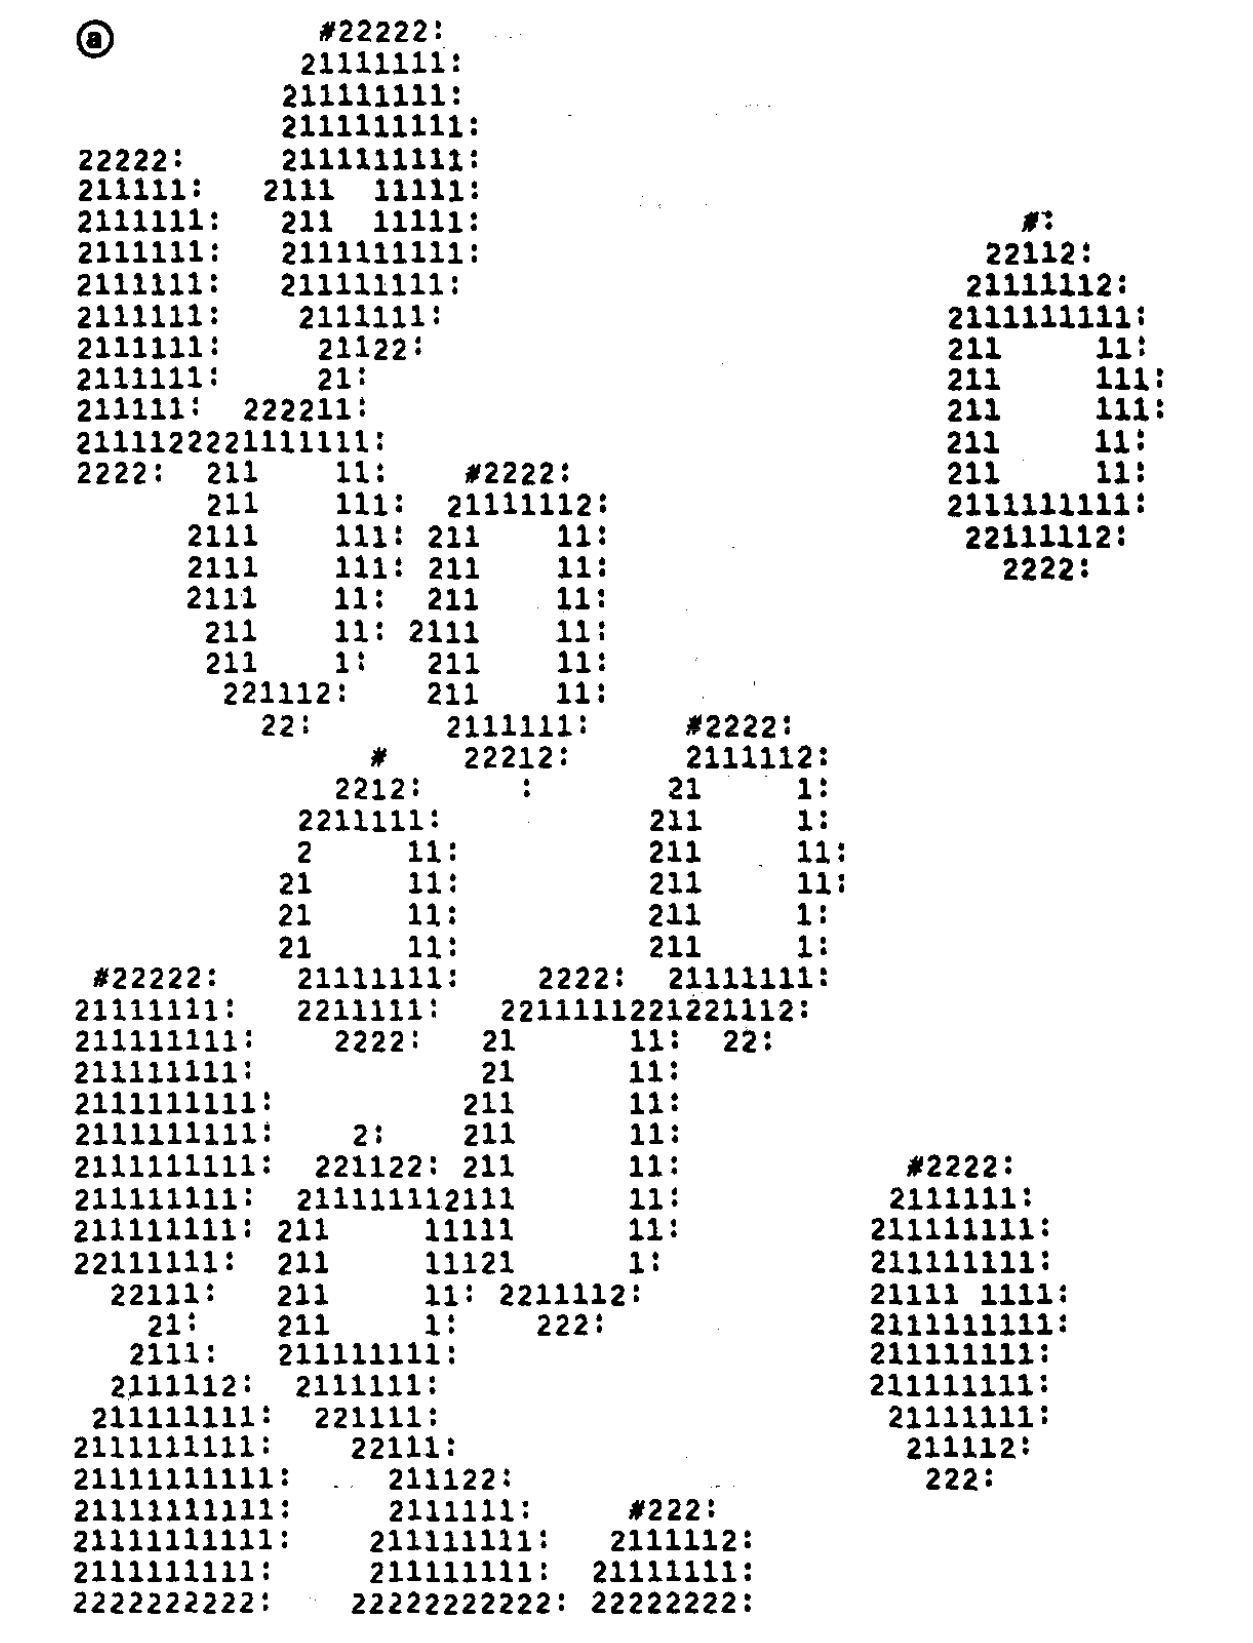
\includegraphics[scale=.15]{a}
\end{figure}
\begin{wrapfigure}{l}{0.4\textwidth}
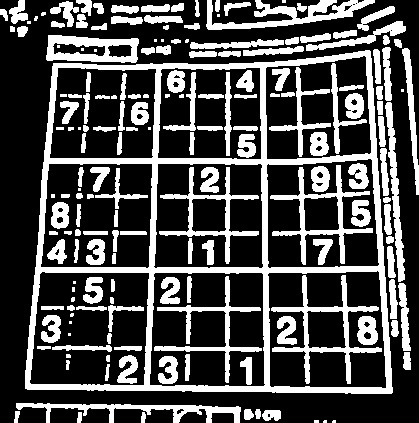
\includegraphics[width=1\linewidth]{filtro}
\caption{Filtro aplicado a un sudoku}
\end{wrapfigure}
Como se puede observar en la imagen los contornos empiezan en el símbolo \# y contin\'uan donde est\'an marcados los
:. El uso de filtros hace que este algoritmo reconozca estos patrones de manera m\'as sencilla, en especial el 
pasar la imagen a un estado binario de forma que quede as\'i:

Haciendo uso de esto podemos conseguir todos los contornos de una imagen de sudoku, al conseguir los contornos
los procesamos haciendo uso del algoritmo de Ramer-Douglas Peucker \cite{ramer} la cual (en resumen) aproxima los puntos
a lineas, las cuales consideraremos como lados, el cual nos permite encontrar todos los cuadrados del sudoku.
Pero como primera instancia debemos de encontrar el cuadrado mas grande, es decir el mas externo.
\vspace{.3cm}
\begin{lstlisting}[style=pythonStyle]
for contour in contours:
         perimeter = cv2.arcLength(contour,True) # largo del contour
         approx = cv2.approxPolyDP(contour, 0.02*perimeter , True) # funcion Ramer, 0.02 es una constante
         if len(approx) == 4: # si es un cuadrado
             if perimeter > maxPerimeter: # para conseguir el contorno mas grande
                 maxPerimeter = perimeter
                 big_square = approx
    return big_square
\end{lstlisting}
Una vez encontrado el contorno m\'as grande nos queda un arreglo con 4 tuplas las cuales representan los puntos
en las esquinas, los cuales usaremos para poder hacer una transformación de perspectiva a la imagen, ya que
como las fotos pueden ser tomadas en \'angulos extra\~nos, se necesita arreglar la perspectiva para que ayude a la
detecci\'on de n\'umeros despu\'es.

\begin{figure}[H]
\centering
\begin{subfigure}{.5\textwidth}
  \centering
  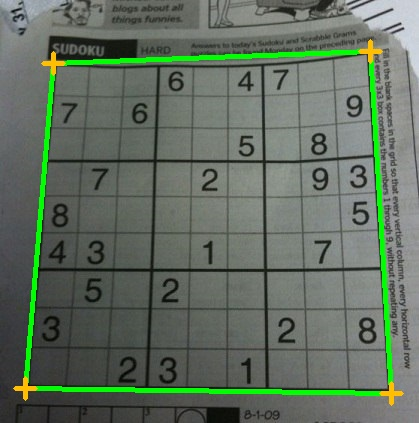
\includegraphics[width=.6\linewidth]{esquinas}
  \caption{Transformaci\'on}
  \label{fig:sub1}
\end{subfigure}%
\begin{subfigure}{.5\textwidth}
  \centering
  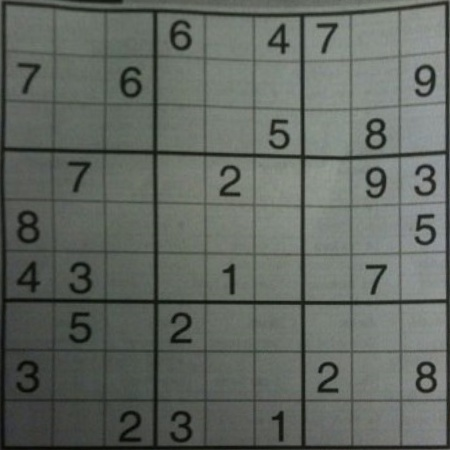
\includegraphics[width=.6\linewidth]{transformada}
  \caption{Esquinas encontradas}
  \label{fig:sub2}
\end{subfigure}
\caption{Procesamiento de imagen}
\label{fig:test}
\end{figure}

Finalmente dividimos el sudoku en sus lineas interiores para poder conseguir
un arreglo de subcuadros, los cuales usaremos para hacer el reconocimiento de 
d\'igitos

\begin{figure}[H]
\caption{Arreglo de subcuadros}
\centering
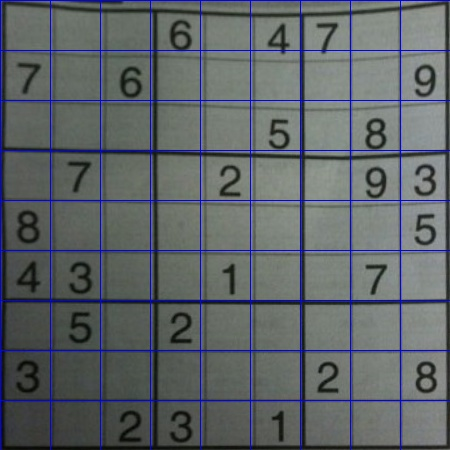
\includegraphics[width=.8\textwidth]{squares}
\end{figure}
% \begin{figure}[h]
% \centering
% \caption{Esquinas de un sudoku}
% 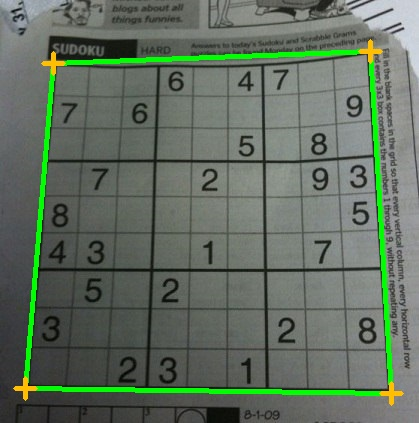
\includegraphics[scale=.3]{esquinas}
% \end{figure}

\subsubsection{Reconocimiento de d\'igitos}
A continuaci\'on, se describir\'a la soluci\'on propuesta para identificar los diferentes n\'umeros encontrados en el tablero del sudoku.
El m\'etodo para la identificaci\'on de los n\'umeros se logra por medio de un modelo que es entrenado por una Red Neuronal Convolucional utilizando el dataset Chars74k. \break
Una red neuronal convolucional es una red que es frecuentemente usada para procesar im\'agenes aprendiendo de relaciones de entrada-salida donde la entrada es una imagen. La operaci\'on b\'asica de una CNN (Red Neuronal Convolucional por sus siglas en ingl\'es) es la convoluci\'on la cual consiste en filtrar una imagen usando una m\'ascara.
\begin{figure}[H]
  \caption{Ejemplo de una convoluci\'on}
  \centering
  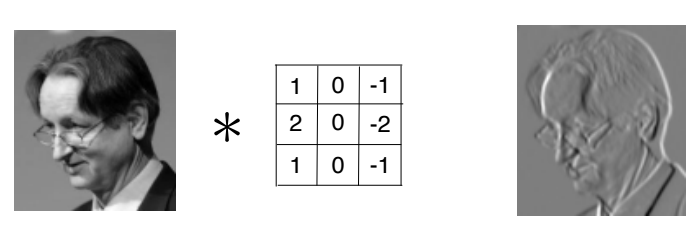
\includegraphics[scale=.50]{convolution}
  \end{figure}

Las 10160 im\'agenes para entrenar a la red fueron tomadas del dataset Chars74K. Estas im\'agenes fueron divididas en el 98\% para el entrenamiento de la red y el restante para realizar la validaci\'on del modelo resultante. Cada una de estas im\'agenes es de fondo negro y contiene un d\'igito del 0 al 9 en color blanco; su tama\~no es de 28x28 pixeles.
\begin{figure}[H]
  \caption{Imagen del dataset Chars74K}
  \centering
  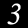
\includegraphics[]{dtimgexample}
\end{figure}

En 1 se puede observar la arquitectura de la red neuronal propuesta para solucionar el problema.
\begin{figure}[H]
  \caption{Arquitectura de la red neuronal construida}
  \centering
  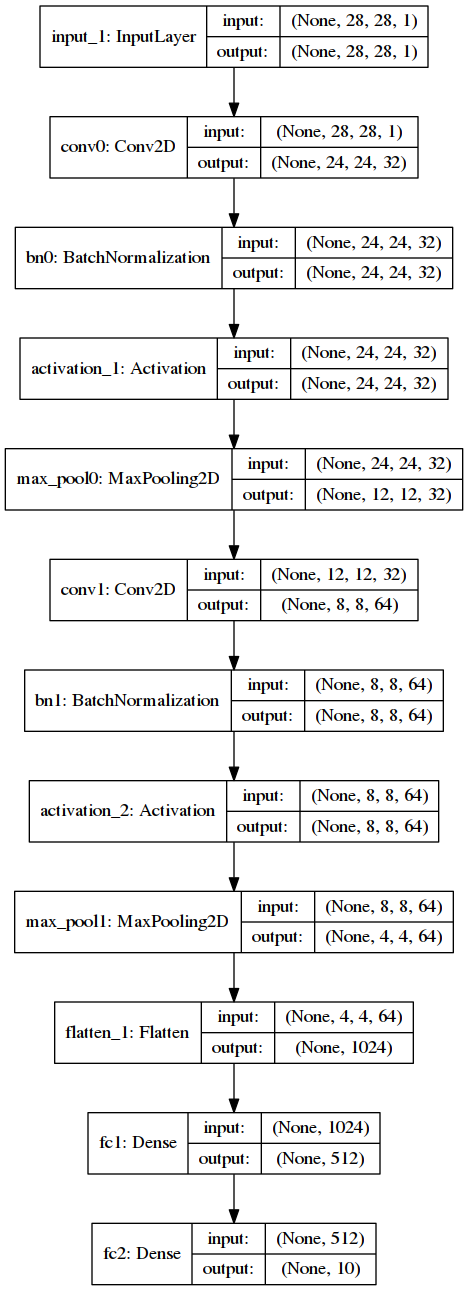
\includegraphics[scale=.40]{model_plot}
\end{figure}
La red neuronal esta compuesta de diferentes capas cada una con un objetivo espec\'ifico.
\paragraph{Capa convolucional} La red construida se compone de dos de \'estas capas, las cuales por medio de filtros se encargan de recorrer las im\'agenes en busca de caracter\'isticas generando un Feature Map.
\begin{figure}[H]
  \caption{Feature map}
  \centering
  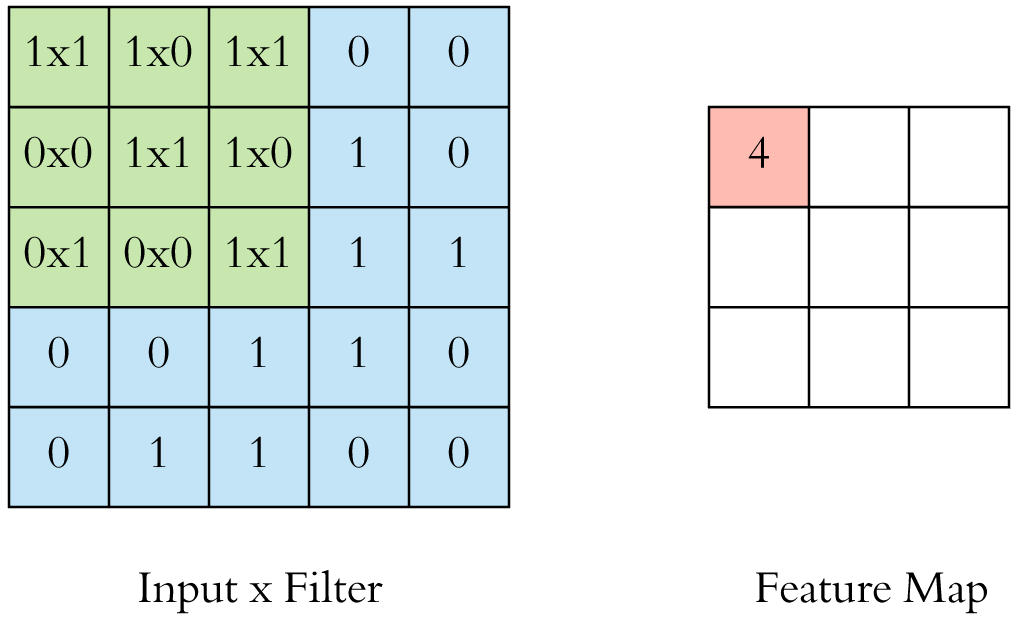
\includegraphics[scale=.20]{feature_map}
\end{figure}
\paragraph{Capa de normalizaci\'on} Para esta capa se usa espec\'ificamente la implementaci\'on de BatchNormalization. Esta capa mantiene los valores que pasan por medio de la red.
\paragraph{Capa de activaci\'on} La red posee dos capas de este tipo cada una con la funci\'on ReLU.
\begin{figure}[H]
  \caption{Funci\'on ReLU}
  \centering
  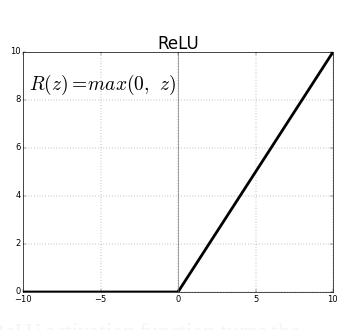
\includegraphics[scale=.40]{relu}
\end{figure}
\paragraph{Capa de pooling} 
Este tipo de capa se encarga de resumir las catarecter\'isticas
obtenidos en los Feature Map generados en la convoluci\'on. 
La configuraci\'on de las capas de pooling recibe como par\'ametros la dimensi\'on de los filtros 
y el stride que define como va a ser recorrido, en este caso, las dimensiones fueron 2x2 y el paso o zancada fue de 1. 
\begin{figure}[H]
  \caption{Comportamiento capa de pooling}
  \centering
  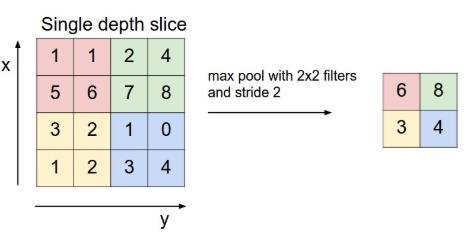
\includegraphics[scale=.80]{pooling}
\end{figure}
\paragraph{Capa de aplanamiento} La capa Flatten se encarga de coger cada una de las matrices y convertirlas en vectores por esto es conocida como capa de aplanamiento.
\begin{figure}[H]
  \caption{Comportamiento capa de aplanamiento}
  \centering
  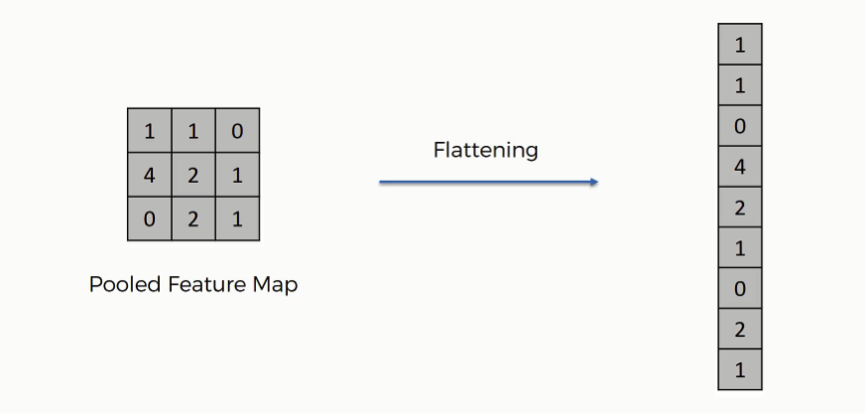
\includegraphics[scale=.80]{flatten}
\end{figure}
\paragraph{Capa completamente conectada (Dense)} Este tipo de capa es tal cual la de una red neuronal b\'asica. En la arquitectura de la red neuronal propuesta se encuentran dos capas de este tipo: Una con 512 neuronas y funci\'on de activaci\'on ReLU y la otra con 10 salidas y funci\'on de activaci\'on softmax.
\begin{figure}[H]
  \caption{Funci\'on Softmax}
  \centering 
  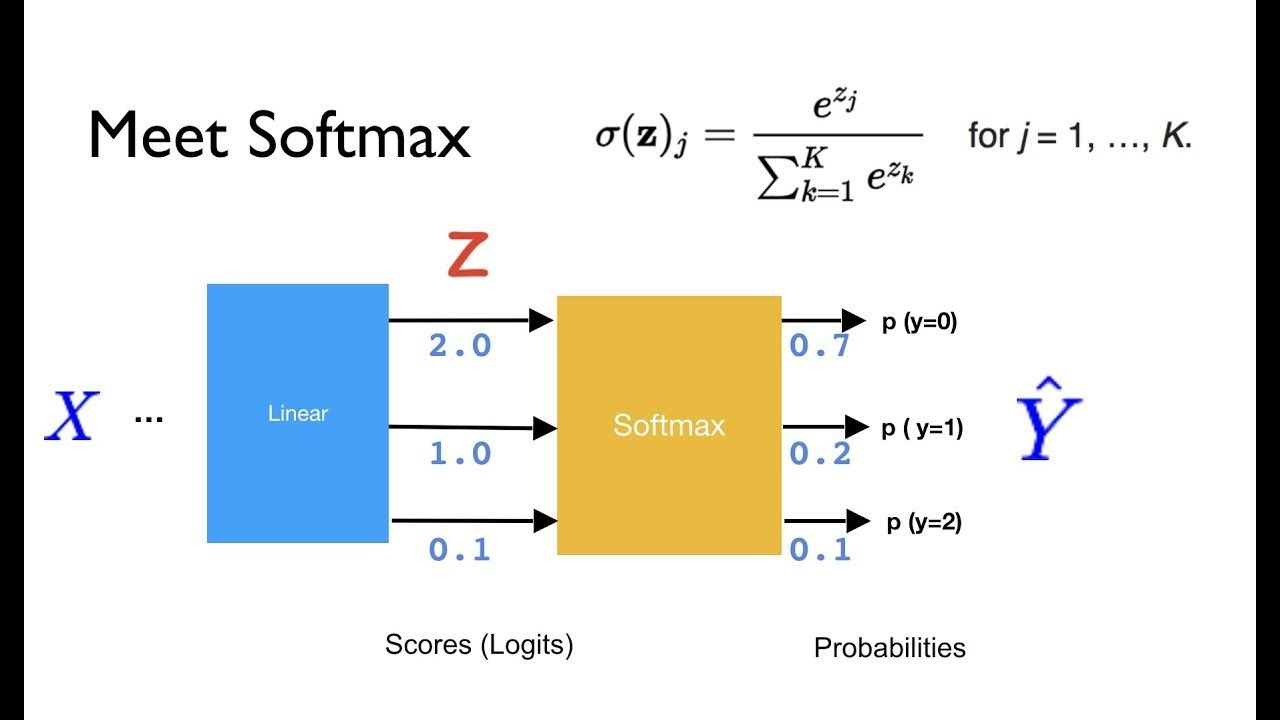
\includegraphics[scale=.30]{softmax}
\end{figure}

Los pesos ser\'an optimizados usando el algoritmo ADAM el cual es un m\'etodo para optimizaci\'on estoc\'astica. La funci\'on de perdida de entrop\'ia cruzada (categorical cross entropy) y las m\'etrica ser\'a accuracy (o taza de acierto).
El entrenamiento fue por medio de lotes , es decir, se actualizaban los par\'ametros internos del modelo cada 83 lotes. La red neuronal fue entrenada por 10 \'epocas.

La red neuronal fue construida usando la libreria Keras la cual trabaja sobre Tensorflow y una vez obtenido el modelo, se puso a disposici\'on por medio de una API REST programada en el lenguaje python bajo el framework Falcon.
\subsubsection{Backtracking}
Una vez identificados los n\'umeros en el tablero para hallar una soluci\'on al sudoku se uso Backtracking el cual es una t\'ecnica de programaci\'on para hacer una b\'usqueda a trav\'es de todas las configuraciones posibles dentro de un espacio de b\'usqueda.
El algoritmo fue programado en el lenguaje de programaci\'on Dart.
\section{Resultados}
Finalmente, se logra la construcci\'on de una aplicaci\'on m\'ovil la cual puede reconocer la disposici\'on de n\'umeros en el tablero del sudoku.
Como trabajo a futuro se podr\'ia mejorar  si se reconocen las celdas donde no hay un d\'igito, ya que, actualmente, esta identificaci\'on se debe hacer de forma manual.
\bibliographystyle{ieeetr}
\bibliography{uni}
    
\end{document}











